\section{Background in Protocols}

In this chapter, each observed protocol is briefly analyzed. Their description focus on explaining how they work, which layer they belong to, and their characteristics. 

This background serves as a base to understand the motivation during experimentation and better comprehend their results.

\subsection{UDP}

The \gls{udp} is a simple message-oriented transport layer protocol that provides a way for application programs to send messages to other programs with a minimum of protocol mechanisms \cite{rfc768}. It has a checksum for data integrity and port numbers for application multiplexing.

Although data integrity can be verified through the checksum, the \gls{udp} is considered an unreliable protocol since it offers no guarantee about delivery or order \cite{data_networks_ip}. Furthermore, there is no need to establish a connection between hosts prior to data transmission, making it a connectionless protocol.

Given the lack of reliability, applications that use \gls{udp} may come across some packet loss, reordering, errors or duplication issues \cite{data_networks_ip}. These applications must provide any necessary confirmation that the data has been received. Nonetheless, \gls{udp} applications usually do not implement any kind of reliability feature, since loss of packets is not usually a problem. Real-time multiplayer games, \gls{voip}, and live streaming are examples of applications that use \gls{udp}.

\subsection{TCP}

In contrast to \gls{udp}’s unreliability, the \gls{tcp} is a connection-oriented protocol designed to provide reliable, ordered, and error-checked transmission of data segments that supports multi-network applications \cite{rfc793}.

\gls{tcp} must be able to deal with incorrect, lost, duplicate, or delivered out of order data to provide reliability \cite{rfc793}. This is achieved by assigning a sequence number to each byte transmitted and requiring an \gls{ack} from the receiver. The sequence number is used to order data that may be received out of order and to eliminate duplicates, and the \gls{ack} ensures data has been delivered, otherwise retransmitted after a given timeout. Finally, incorrect data is handled by adding a checksum to each segment transmitted, and discarding any incorrect segments.

To be able to control the amount of data sent by the sender, \gls{tcp} returns a “window” with every \gls{ack} indicating the range of acceptable segments beyond the last successfully received segment \cite{rfc793}. Therefore, the window specifies the number of bytes that the receiver is willing to receive.

Since \gls{tcp} is connection-oriented, it needs to keep certain status information about the data stream to ensure reliability and flow control. A connection is defined as a set of information about the transfer, including sockets, sequence numbers, and window sizes. Each connection is distinguished by a pair of sockets between the two hosts. To initiate a connection, the  \gls{tcp} uses a three-way handshake (Figure 1) to establish a reliable connection \cite{telecom_network_security}.

\begin{figure}[ht]
    \centering
    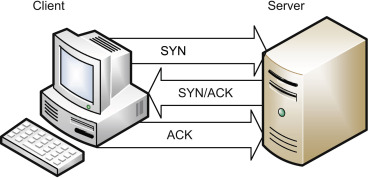
\includegraphics[width=\linewidth]{figures/3-s2.0-B9780128024379000059-f05-08-9780128024379.jpg}
    \caption{TCP Three-Way Handshake}
    {Source: \cite{telecom_network_security}}
    \label{figure:tcp_handshake}
\end{figure}

The sender chooses the initial sequence number, informed in the first \gls{syn} packet. The receiver also chooses its own initial sequence number by informing in the \gls{synack} sent to the sender. Each side acknowledges each other’s sequence number by incrementing it, allowing both sides to detect missing or out-of-order segments \cite{telecom_network_security}.

\gls{tcp} is stream oriented, effectively meaning it has the ability to send or receive a stream of bytes \cite{rfc793}. It can bundle up data that comes from the application layer and send it in a single segment, being responsible for breaking the stream of data into segments, and reassembling once they reach the other side. \gls{udp}, on the contrary, is a message-oriented protocol where the division of data into user datagrams is made by the application \cite{data_networks_ip}.

To be able to offer more functionality, \gls{tcp} ends up sacrificing efficiency. While in the case of a connectionless and unreliable protocol such as \gls{udp}, it turns out to be faster due to the lack of any extra features \cite{tcp_udp_comparison}.

\subsection{TLS}

As more people have access to the Internet, the higher the requirement is for it to be secure. Data generated by users can have many harmful implications since it is directly related to privacy. While offering reliability, which is a necessary attribute to Internet’s communication, \gls{tcp}’s communication is not encrypted. Therefore, anyone with a minimum knowledge of networking can see everything that’s traversing the network, breaking with users' privacy.

The \gls{tls} protocol is a cryptographic protocol designed to provide privacy and data integrity between two communicating applications \cite{rfc5246}. The connection is considered private since symmetric cryptography is used for data encryption and every connection has an unique generated key negotiated between parties.

Peers' identity can be authenticated through the use of asymmetric cryptography \cite{auto_verification_tls_handshake}. This is important because both sender and receiver can establish a trusted relationship by verifying if their certificates and public IDs are valid and have been issued by a \gls{ca} listed in their respective list of trusted \gls{ca}s.

To be able to establish a \gls{tls} connection, the sender and receiver must negotiate a connection by doing a \gls{tls} handshake. It allows hosts to authenticate with each other and to negotiate a cipher and generate session keys in order to use symmetric encryption before the application protocol actually starts to transmit data.

\gls{tls} can be used to encrypt \gls{tcp} connections by including the \gls{tls} handshake to \gls{tcp}’s connection establishment flow (Figure \ref{figure:tls_handshake}). This adds an overhead by increasing the number of \gls{rtt} needed before the actual data transmission starts.

\begin{figure}[ht]
    \centering
    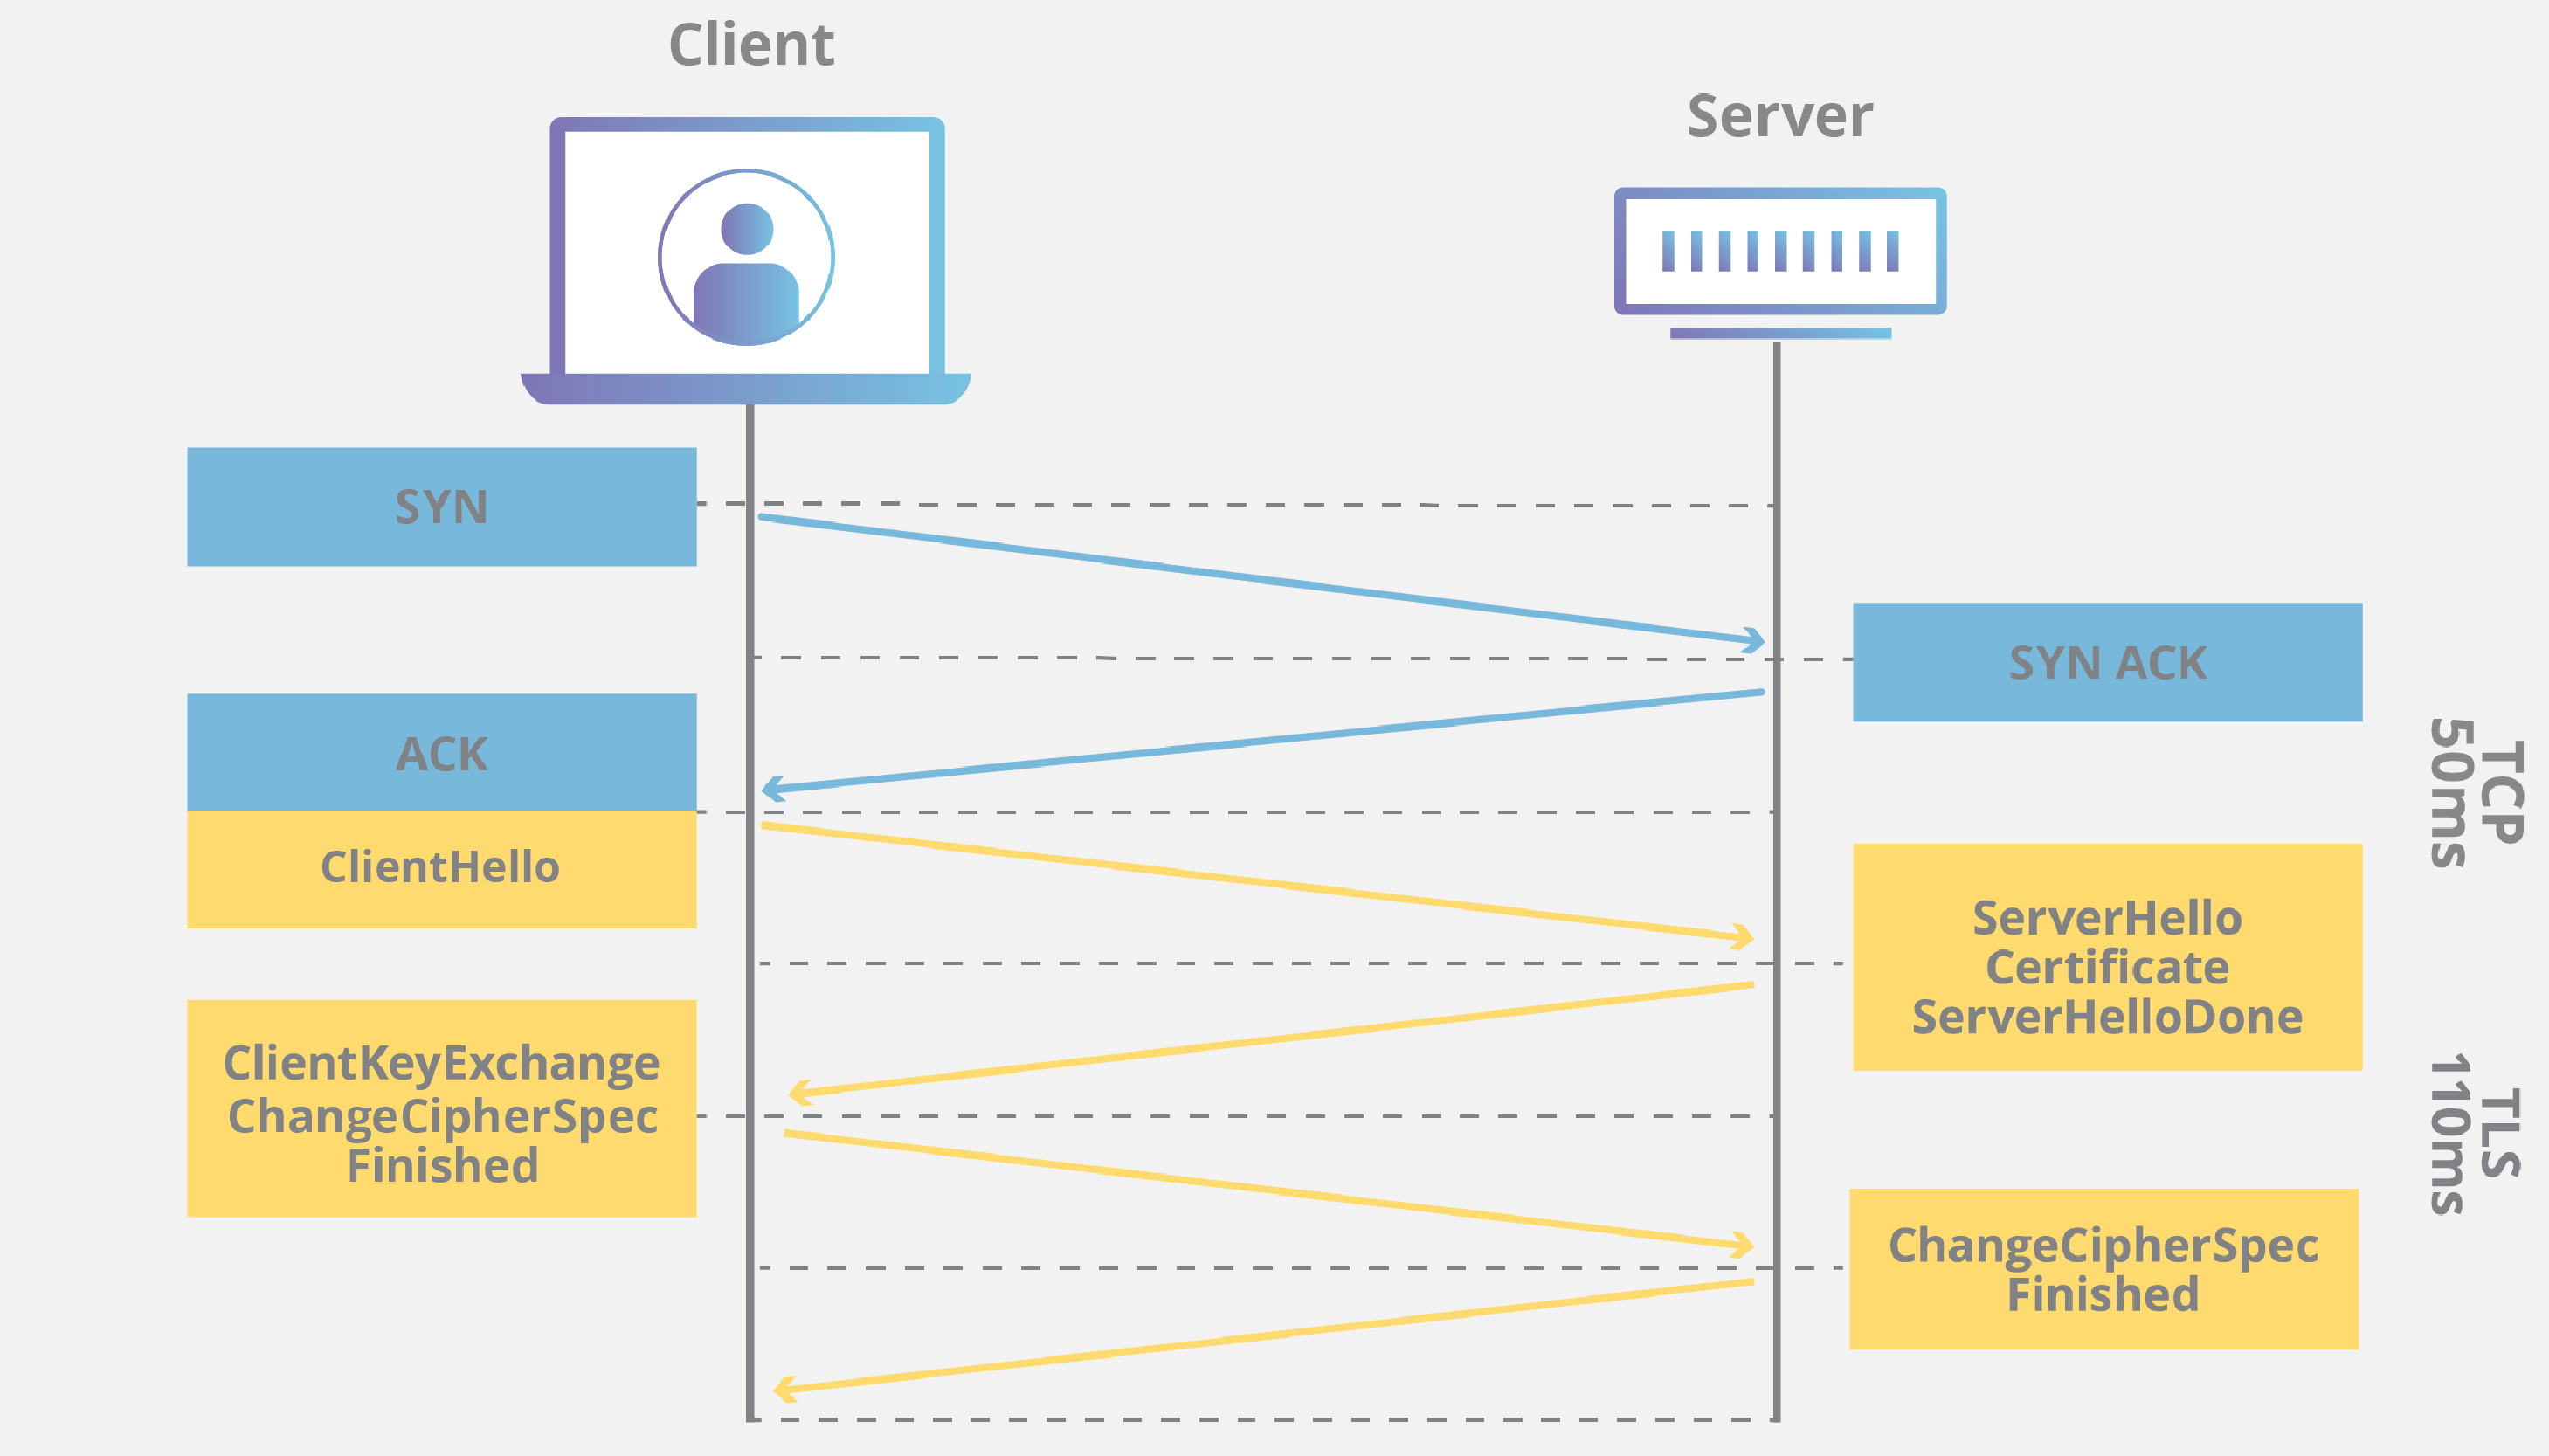
\includegraphics[width=\linewidth]{figures/tls-ssl-handshake.png}
    \caption{TLS Handshake}
    {Source: \cite{what_is_a_tls_handshake}}
    \label{figure:tls_handshake}
\end{figure}

Working alongside one another, \gls{tcp} and \gls{tls} have kept the Internet reliable and encrypted. However, they only provide the channel of communication, how applications communicate is determined by the application-layer protocols.

\subsection{HTTP}

The \gls{http} is considered the foundation of the World Wide Web. It is an application-level protocol for distributed, collaborative, hypermedia information systems that runs on top of the other layers in the network protocol stack \cite{rfc1945, rfc2616, what_is_http}.

It is a generic, stateless protocol which uses a predefined set of standards and rules for exchange of information through a request-response process \cite{rfc1945, rfc2616}. The sender submits an \gls{http} request message to the receiver, which provides resources, such as \gls{html}, or performs some action on behalf of the sender. The receiver then returns a response message to the sender, it contains status information about the request and possibly the requested data in the message body, enabling the sender to react in a proper way, either by moving on to another task or handling an error \cite{rfc2616}.

The following subsections introduce \gls{http} versions, what they improved and a general feeling of how they work.

\subsection{HTTP/1}

The first version of \gls{http}, known as \gls{http}/0.9, was a simple protocol for raw data transfer across the Internet \cite{rfc2616}. It only had the GET request method, equivalent to a request to retrieve data from the server. Message types were limited to text, and it had no \gls{http} headers, meaning there was no metadata, such as status or error codes, on the request/response.

\gls{http}/1.0 improved the protocol by allowing messages to support the \gls{mime} standard, which extends data types supported by messages, being possible to send videos, audio, and images \cite{rfc2616}. In addition, metadata was also incorporated into requests and responses, increasing the available request methods, while improving error handling by the use of status and error codes.

\gls{http}/1.1 is considered a milestone in the evolution of the Internet, since it eliminates a lot of problems from previous versions and introduces a series of optimizations \cite{what_is_http}. Connections can be reused in favour of having to create a connection to every request and can be pipelined, improving the time needed to perform multiple requests. It also provides support for chunked transfer, which is a streaming data transfer mechanism that divides the data stream into “chunks” that are sent out independently of each other. This allowed for a more efficient transfer of large amounts of data due to concurrency.

\subsection{HTTP/2}

\gls{http}/2 purpose is to optimize transport for \gls{http} semantics, while keeping the support for all of the core features of the \gls{http}/1.1.

Even though \gls{http}/1.1 added pipelined connections, it still suffers from the Head of Line blocking (HOL blocking) problem \cite{rfc7540}. It happens when the number of allowed parallel requests is used up, and subsequent requests need to wait for the former ones to complete. \gls{http}/2 solves this by implementing multiplexing. This is achieved by having \gls{http} request/response associated with its own stream and since streams are independent of each other, a blocked request/response does not prevent progress on other streams.

\gls{http}/2 adds a new interaction mode where a receiver can push responses to the sender \cite{rfc7540}. This resulted in senders not needing to send periodical requests for new data to the server by using polling methods, trading network usage for some improvement in latency.

Because \gls{http} header can contain a lot of redundant data, \gls{http}/2 uses a compressed binary representation of metadata instead of a textual one, this reduces the space required \cite{rfc7540}.

\subsection{HTTPS}

\gls{https} is an extension of \gls{http}, conceptually equivalent to \gls{http} over \gls{tls} \cite{rfc2818}. \gls{https} is when the \gls{http} client also acts as a \gls{tls} client, it should perform all \gls{tls} requirements, such as establishing a connection through a \gls{tls} handshake. Once it finishes, the client may initiate the first \gls{http} request, the difference being all data will be encrypted. \gls{https} maintains \gls{http} behaviour while providing \gls{tls} features for instance encryption, data integrity, and authentication \cite{rfc2818}.

\subsection{QUIC}

\gls{https} provides a reliable and secure connection and is considered the main application-layer protocol used by the World Wide Web. However, it has some limitations due to requiring the use of \gls{tls} for security and \gls{tcp} for reliability.

QUIC is a secure general-purpose transport protocol designed to improve performance for \gls{https} traffic and to enable rapid deployment and continued evolution of transport mechanisms \cite{quic_protocol}. It replaces most of the traditional \gls{https} stack: \gls{http}/2. \gls{tls}, and \gls{tcp} (Figure \ref{figure:quic_http2_layers}).

\begin{figure}[ht]
    \centering
    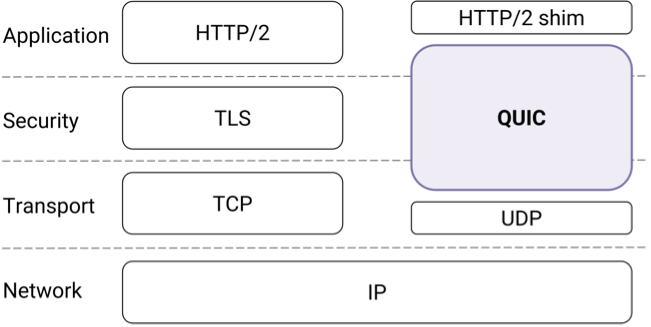
\includegraphics[width=\linewidth]{figures/Introduction.png}
    \caption{QUIC in the traditional HTTPS stack}
    {Source: \cite{quic_protocol}}
    \label{figure:quic_http2_layers}
\end{figure}

As the Internet evolves, software requires fast deployment of changes both to improve and to secure it. \gls{tcp} is a kernel-space transport protocol, meaning that any vulnerabilities or improvements require an upgrade to the \gls{os} kernel. Since such changes have a huge impact on the entire system, they must be made with caution and may take years to become widely spread \cite{rfc9000}. QUIC was developed as a user-space transport protocol on top of \gls{udp}, facilitating its deployment as part of other applications, resulting in meaningful impact in a relatively short time \cite{quic_protocol}.

A middlebox is when a device adds functionality other than packet forwarding to an IP router, such as filtering, altering, and manipulating traffic \cite{rfc3234}. Improvements to transport protocols is reduced due to the fact that these kinds of devices are hard to be removed or upgraded, creating a dependency between them. For example, firewalls tend to block any unknown traffic for security reasons, meaning that new transport protocols need to be explicitly supported \cite{rfc3234}. QUIC addresses this issue by encrypting its packets, therefore avoiding middlebox dependency and data tampering \cite{quic_protocol}.

\gls{http}/2 solves the HOL blocking problem in the application layer by introducing request multiplexing, however it still suffers from this problem in the transport layer. Even though \gls{http}/2 streams are independent of each other, they still had to share a \gls{tcp} connection and deal with \gls{tcp}’s window size. If the first window segment fails, the window cannot go further and blocks new segments from being transmitted. QUIC solves this problem by implementing stream multiplexing. More than one stream within a connection means that even if one stream drops packets, other streams will not be blocked in any way.

\gls{https} is required to perform both \gls{tcp} and \gls{tls} handshakes to establish a secure connection, resulting in generally a 3-\gls{rtt} connection setup (Figure \ref{figure:tcp_v_tls_v_quic_handshake}) to be able to start transmitting the actual data \cite{rfc7413}.

\begin{figure}[ht]
    \centering
    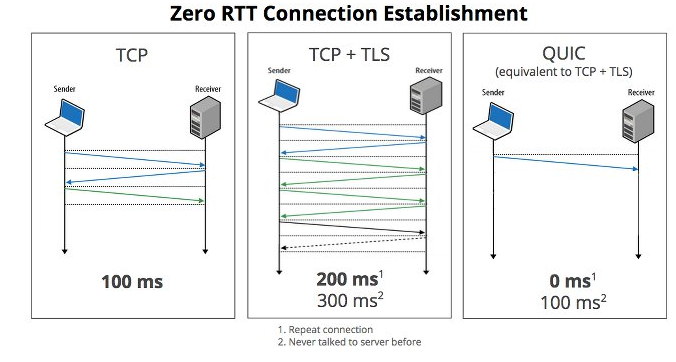
\includegraphics[width=\linewidth]{figures/quic_zerortt.png}
    \caption{Zero RT Connection Establishment}
    {Source: \cite{google_edge_network}}
    \label{figure:tcp_v_tls_v_quic_handshake}
\end{figure}

QUIC improves the handshake delay by minimizing the steps required to establish a connection, being able to perform a 0-\gls{rtt} connection setup once the server is known (Figure \ref{figure:quic_handshake}) \cite{quic_protocol, rfc9000}. It does this by caching information about the server on the client after a successful connection. If it tries to set up a connection with expired information, the server sends a reject message that contains all the information necessary to establish a connection.

\begin{figure}[ht]
    \centering
    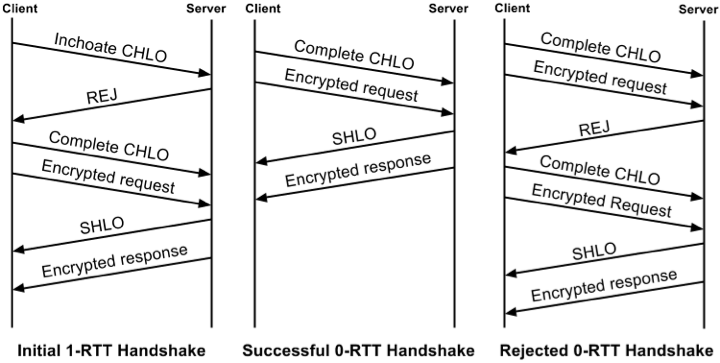
\includegraphics[width=\linewidth]{figures/ConnectionEstablishment.png}
    \caption{Timeline of QUIC’s initial 1-RTT handshake, a subsequent successful 0-RTT handshake, and a failed 0-RTT handshake}
    {Source: \cite{quic_protocol}}
    \label{figure:quic_handshake}
\end{figure}

\gls{tcp} loss recovery mechanisms are able to detect when a segment is probably dropped, triggering its retransmission. This process uses \gls{rtt} estimation to improve its efficiency, which in the case of \gls{tcp}, is based on \gls{tcp}’s sequence numbers. However, once a retransmission is made, there is no way of knowing if the \gls{ack} received is for the original or the retransmitted segment since both segments use the same sequence number. Additionally, dropped retransmission segments are usually detected by the use of timeouts, further slowing \gls{tcp} \cite{quic_protocol,rfc2988,rfc9000,tcp_timer_dont_work_well}.

QUIC eliminates \gls{tcp}’s retransmission ambiguity problem by including a new packet number to all packets, even those including retransmitted data \cite{rfc9000}. This means it can measure \gls{rtt}s precisely since it always knows which packet each \gls{ack} refers to. To maintain the data order, QUIC adds a stream offset to the stream frames present in the packet, decoupling the need of ordered packet numbers \cite{quic_protocol}.

While QUIC improves transport efficiency, it demands more computational resources when compared to \gls{tcp}+\gls{tls}. The focus during its design was improving transport, not resource efficiency, resulting in an initial raise by 3.5 times of \gls{cpu} utilization when compared to \gls{tcp}+\gls{tls} traffic \cite{quic_protocol}. Optimizations were made after this assessment, decreasing \gls{cpu} usage difference to 2 times \gls{tcp}+\gls{tls}’.

\subsection{HTTP/3}

\gls{http}/3 is effectively \gls{http} over QUIC. It provides a transport for \gls{http} semantics using QUIC as transport protocol, therefore it maintains all the same request methods, status codes, and messages fields. It still does not have an official \gls{rfc}, however it possesses an initial draft [32]. Nonetheless, it is supported by 74\% of running web browsers, Google Chrome being one of them [33].

\subsection{Summary}

This section went over the important aspects of each transport-layer and application-layer protocols experimented throughout this study. Therefore, their differences should be clear, as well as what they try to improve.

The next section will explore a few aspects of distributed systems on cloud environment. These systems makes extensive use of the observed protocols as a way of communicating with each other. Without them, however, they would not be able to talk to each other and achieve cooperation.
